\documentclass[12pt,a4paper]{article}

% ── Encoding and Language ──
\usepackage[utf8]{inputenc}
\usepackage[T1]{fontenc}
\usepackage[spanish]{babel}

% ── Layout ──
\usepackage[a4paper, margin=2.5cm]{geometry}
\usepackage{fancyhdr}
\usepackage{setspace}
\usepackage{placeins}
\onehalfspacing

% ── Typography ──
\usepackage{lmodern}
\usepackage{microtype}

% ── Graphics and TikZ ──
\usepackage{graphicx}
\usepackage{tikz}
\usetikzlibrary{positioning, arrows, shapes.geometric, arrows.meta, calc, fit, backgrounds}

% ── Colors ──
\usepackage{xcolor}
\definecolor{codebg}{rgb}{0.96,0.96,0.96}
\definecolor{codecomment}{rgb}{0.4,0.6,0.4}
\definecolor{codekeyword}{rgb}{0.2,0.4,0.8}
\definecolor{codestring}{rgb}{0.8,0.3,0.3}
\definecolor{codenumber}{rgb}{0.5,0.5,0.5}

% ── Code ──
\usepackage{listings}
\lstdefinestyle{javastyle}{
    backgroundcolor=\color{codebg},
    commentstyle=\color{codecomment}\itshape,
    keywordstyle=\color{codekeyword}\bfseries,
    numberstyle=\tiny\color{codenumber},
    stringstyle=\color{codestring},
    basicstyle=\ttfamily\footnotesize,
    breaklines=true,
    captionpos=b,
    keepspaces=true,
    numbers=left,
    numbersep=8pt,
    showspaces=false,
    showstringspaces=false,
    tabsize=4,
    frame=single,
    rulecolor=\color{black!20},
    language=Java
}
\lstset{style=javastyle}

% ── Tables ──
\usepackage{booktabs}
\usepackage{array}
\usepackage{tabularx}

% ── Boxes ──
\usepackage{float}
\usepackage{tcolorbox}

% ── Links ──
\usepackage[
    colorlinks=true,
    linkcolor=black,
    urlcolor=gray,
    citecolor=gray
]{hyperref}

% ── Document variables ──
\newcommand{\subject}{Programación Avanzada}
\newcommand{\titlecourse}{Sistema de Gestión Universitaria}
\newcommand{\university}{Universidad del Aconcagua}
\newcommand{\faculty}{Facultad de Ciencias Sociales y Administrativas}
\newcommand{\repourl}{https://github.com/AxelMrak/proyecto\_final\_prog\_avanzada}

% ── Header and Footer ──
\pagestyle{fancy}
\fancyhf{}
\lhead{\textit{\titlecourse}}
\rhead{\textit{\subject}}
\rfoot{\thepage}
\setlength{\headheight}{15pt}

\begin{document}

% ======================================================================
% PORTADA
% ======================================================================
\begin{titlepage}
    \centering
    \vspace*{3cm}

    {\Large \textbf{\university}}\\[0.5cm]
    {\large \faculty}\\[2cm]

    {\Huge \textbf{\titlecourse}}\\[0.5cm]
    {\Large \subject\ --- Proyecto Final}\\[2cm]

    \rule{0.8\textwidth}{0.5pt}\\[0.5cm]

    {\large \textbf{Integrantes:}}\\[0.4cm]
    {\large Axel Sarmiento}\\[0.2cm]
    {\large Julián Molina}\\[0.2cm]
    {\large Andrés Riveros}\\[0.5cm]

    {\large \today}\\[0.8cm]

    {\small Repositorio: \href{\repourl}{\texttt{\repourl}}}

    \vfill
\end{titlepage}

% ======================================================================
% ÍNDICE
% ======================================================================
\tableofcontents
\newpage

% ======================================================================
% 1. RESUMEN
% ======================================================================
\section{Resumen}

El presente informe documenta el desarrollo del \textbf{Sistema de Gestión
Universitaria}, una aplicación de consola en Java~17 que administra alumnos,
docentes, administrativos, materias e inscripciones de una universidad. La
aplicación permite dar de alta usuarios, inscribir alumnos en materias, y que
los docentes carguen notas finales, todo respaldado por una base de datos
SQLite con esquema normalizado.

El proyecto se destaca por haber sido diseñado desde el inicio con una
\emph{arquitectura limpia} en cuatro capas — dominio, aplicación,
infraestructura y presentación — y por aplicar los principios \textbf{SOLID}
de forma deliberada. La capa de dominio está completamente aislada de
detalles de infraestructura (JDBC, SQLite), las interfaces de repositorio
respetan el \emph{Interface Segregation Principle}, y la inyección de
dependencias se realiza manualmente en el punto de entrada.

El sistema se ejecuta desde terminal, con un menú interactivo que valida
cada campo en el momento del ingreso y ofrece listas numeradas para
seleccionar alumnos y materias sin necesidad de memorizar legajos o códigos.

\paragraph{Palabras clave:} Java~17, SQLite, JDBC, arquitectura limpia,
SOLID, Maven, aplicación de consola.

% ======================================================================
% 2. INTRODUCCIÓN
% ======================================================================
\section{Introducción}

\subsection{Contexto}

La cátedra de \textbf{Programación Avanzada} propone como trabajo final el
desarrollo de un sistema de información en Java que aplique los conceptos de
la materia: diseño orientado a objetos, persistencia con base de datos,
separación de responsabilidades, principios SOLID y documentación
profesional. El equipo seleccionó un sistema de gestión universitaria por su
riqueza de entidades (usuarios con distintos roles, materias, inscripciones,
notas) y porque permite demostrar la aplicación de patrones de diseño en un
dominio realista.

\subsection{Objetivos}

\begin{itemize}
    \item Implementar un sistema de consola funcional para la gestión de
        alumnos, docentes, administrativos, materias e inscripciones.
    \item Diseñar una \textbf{arquitectura en capas} que separe el dominio
        de la infraestructura y de la presentación.
    \item Normalizar el esquema de base de datos a tercera forma normal
        (3NF) con restricciones CHECK e índices sobre claves foráneas.
    \item Aplicar los principios \textbf{SOLID}, en particular SRP, ISP y
        DIP.
    \item Validar cada entrada del usuario en el momento del ingreso, sin
        postergar errores al final del formulario.
    \item Entregar un informe profesional y un repositorio público con
        control de versiones.
\end{itemize}

\subsection{Alcance}

El proyecto comprende:
\begin{itemize}
    \item El código fuente completo del sistema (33 archivos Java).
    \item Scripts SQL de migración (DDL + datos semilla).
    \item Un test de integración que verifica 25 casos (validadores,
        constructores, carga de nota, persistencia).
    \item El presente informe en \LaTeX{} (compilable a PDF).
    \item Repositorio remoto: \href{\repourl}{\texttt{\repourl}}.
    \item Videos demostrativos y capturas de pantalla en la carpeta
        \texttt{Recursos/}.
\end{itemize}

% ======================================================================
% 3. DESCRIPCIÓN DEL PROYECTO
% ======================================================================
\section{Descripción del Proyecto}

\subsection{Concepto}

El \textbf{Sistema de Gestión Universitaria} es una aplicación de línea de
comandos que modela las operaciones habituales de una facultad. Un menú
principal da acceso a tres submódulos: Alumnos, Docentes y
Administrativos.

\subsection{Funcionalidades}

\begin{itemize}
    \item \textbf{Alta de usuarios:} registro de alumnos (con carrera y año
        de ingreso), docentes (con departamento y categoría) y
        administrativos (con sector).
    \item \textbf{Listado:} consulta tabulada de cada tipo de usuario, con
        sus datos completos.
    \item \textbf{Inscripción a materias:} desde el menú de Alumnos, se
        selecciona un alumno (por legajo o eligiendo de una lista numerada)
        y una materia (por código o lista), y se registra la inscripción.
    \item \textbf{Carga de notas:} desde el menú de Docentes, se selecciona
        un alumno y una materia de listas desplegables, se ingresa una nota
        (0--10) y se persiste en la base de datos. El sistema valida que el
        alumno exista, que la materia exista y que el alumno esté inscripto
        en ella.
    \item \textbf{Validación por campo:} cada campo (nombre, legajo, email,
        año, nota) se valida en el momento de ingreso; si falla, se
        re-pregunta el mismo campo sin perder los anteriores.
\end{itemize}

\subsection{Capturas del sistema}

Las siguientes capturas, incluidas en la carpeta \texttt{Recursos/},
muestran el sistema en funcionamiento durante distintas operaciones.

\begin{figure}[H]
    \centering
    \includegraphics[width=0.75\textwidth]{../Recursos/interaccion-app1.png}
    \label{fig:app1}
\end{figure}

\begin{figure}[H]
    \centering
    \includegraphics[width=0.75\textwidth]{../Recursos/interaccion-app3.png}
    \label{fig:app3}
\end{figure}

\begin{figure}[H]
    \centering
    \includegraphics[width=0.75\textwidth]{../Recursos/interaccion-app5.png}
    \label{fig:app5}
\end{figure}

% ======================================================================
% 4. TECNOLOGÍAS UTILIZADAS
% ======================================================================
\section{Tecnologías Utilizadas}

\begin{itemize}
    \item \textbf{Java~17} --- lenguaje de programación principal. Se usa
        \texttt{var} para inferencia de tipos locales, \texttt{switch}
        expressions, \texttt{record} y streams.
    \item \textbf{Maven~3} --- gestor de construcción y dependencias. El
        plugin \emph{maven-shade-plugin} empaqueta un JAR auto-contenido
        (fat JAR) con todas las dependencias.
    \item \textbf{SQLite~3 (JDBC)} --- motor de base de datos embebido.
        Cero configuración: la base se crea automáticamente al iniciar la
        aplicación.
    \item \textbf{Git} --- control de versiones. Repositorio público en
        GitHub.
    \item \textbf{\LaTeX{}} --- sistema de composición tipográfica para
        este informe.
\end{itemize}

\begin{figure}[h]
    \centering
    \begin{tikzpicture}[
        box/.style={draw, rounded corners, minimum width=5cm,
                    minimum height=0.7cm, align=center},
    ]
        \node[box, fill=blue!5]  (latex) at (0, 0)   {\LaTeX};
        \node[box, fill=blue!10] (git)   at (0,-0.9) {Git};
        \node[box, fill=blue!15] (mvn)   at (0,-1.8) {Maven + Shade Plugin};
        \node[box, fill=blue!20] (jdbc)  at (0,-2.7) {SQLite (JDBC)};
        \node[box, fill=blue!25] (java)  at (0,-3.6) {Java 17};
    \end{tikzpicture}
    \caption{Stack tecnológico. Cada capa se apoya sobre la de abajo: la
    aplicación corre sobre Java, que accede a SQLite vía JDBC; Maven
    construye y empaqueta; Git versiona; \LaTeX{} produce el informe.}
\end{figure}

% ======================================================================
% 5. ARQUITECTURA DEL SOFTWARE
% ======================================================================
\section{Arquitectura del Software}

\subsection{Arquitectura limpia en cuatro capas}

El sistema se organiza en cuatro capas con dependencias unidireccionales:
la capa de dominio no conoce a ninguna otra; la de aplicación conoce al
dominio; la de infraestructura implementa las interfaces del dominio; y
la de presentación consume los servicios de aplicación.

\begin{itemize}
    \item \textbf{domain/} --- Entidades de negocio (\texttt{Estudiante},
        \texttt{Docente}, \texttt{Administrativo}, \texttt{Materia},
        \texttt{Inscripcion}), \emph{value objects} (\texttt{Nota}),
        enumeraciones con id de base de datos (\texttt{Rol},
        \texttt{CategoriaDocente}, \texttt{EstadoInscripcion}) y las
        interfaces de repositorio que definen \emph{qué} operaciones de
        persistencia necesita el dominio, sin decir \emph{cómo}.
    \item \textbf{application/} --- Servicios de caso de uso:
        \texttt{EstudianteService}, \texttt{DocenteService},
        \texttt{AdministrativoService}, \texttt{InscripcionService}.
        Orquestan las reglas de negocio (validar existencia, verificar
        inscripción previa, cargar nota) y delegan la persistencia a las
        interfaces del dominio.
    \item \textbf{infrastructure/} --- Implementaciones concretas:
        \texttt{ConnectionFactory} (abre conexiones JDBC a SQLite), cinco
        repositorios JDBC que implementan las interfaces del dominio, y
        \texttt{Migrator} (ejecuta los scripts \texttt{.sql} en orden sobre
        el arranque).
    \item \textbf{ui/menu/} --- Menús de consola (\texttt{MenuAlumnos},
        \texttt{MenuDocentes}, \texttt{MenuAdministrativos}). Cada menú
        recibe sus dependencias por constructor y coordina la interacción
        con el usuario vía \texttt{InputReader}.
\end{itemize}

\subsection{Diagrama de capas}

\begin{figure}[!htbp]
    \centering
    \begin{tikzpicture}[
        node distance=0.8cm,
        layer/.style={draw, rounded corners, minimum width=6.5cm,
                      minimum height=0.9cm, align=center, thick},
        arrow/.style={-{Latex[length=3mm]}, thick},
    ]
        \node[layer, fill=yellow!15] (ui)
            {\textbf{ui/menu/} \hspace{0.5cm} (presentación)\\
             \small MenúAlumnos \quad MenúDocentes \quad MenúAdministrativos};

        \node[layer, fill=green!12, below=of ui] (app)
            {\textbf{application/} \hspace{0.5cm} (casos de uso)\\
             \small Servicios: Estudiante, Docente, Administrativo, Inscripción};

        \node[layer, fill=blue!10, below=of app] (domain)
            {\textbf{domain/} \hspace{0.5cm} (reglas de negocio)\\
             \small Entidades, Value Objects, Enums, Repository Interfaces};

        \node[layer, fill=red!10, below=of domain] (infra)
            {\textbf{infrastructure/} \hspace{0.5cm} (detalles técnicos)\\
             \small JDBC Repositories, ConnectionFactory, Migrator};

        \draw[arrow] (ui)    -- node[right, font=\small\itshape] {llama}   (app);
        \draw[arrow] (app)   -- node[right, font=\small\itshape] {usa}     (domain);
        \draw[arrow] (infra) -- node[left,  font=\small\itshape] {implementa} (domain);
    \end{tikzpicture}
    \caption{Las cuatro capas del sistema. La UI llama a los servicios de
    aplicación; éstos usan el dominio (entidades + reglas); la
    infraestructura implementa las interfaces que el dominio declara. La
    capa de dominio no conoce nada por debajo de ella.}
\end{figure}

\subsection{Diagrama UML de clases}

El siguiente diagrama muestra las entidades principales y sus relaciones.

\begin{figure}[H]
    \centering
    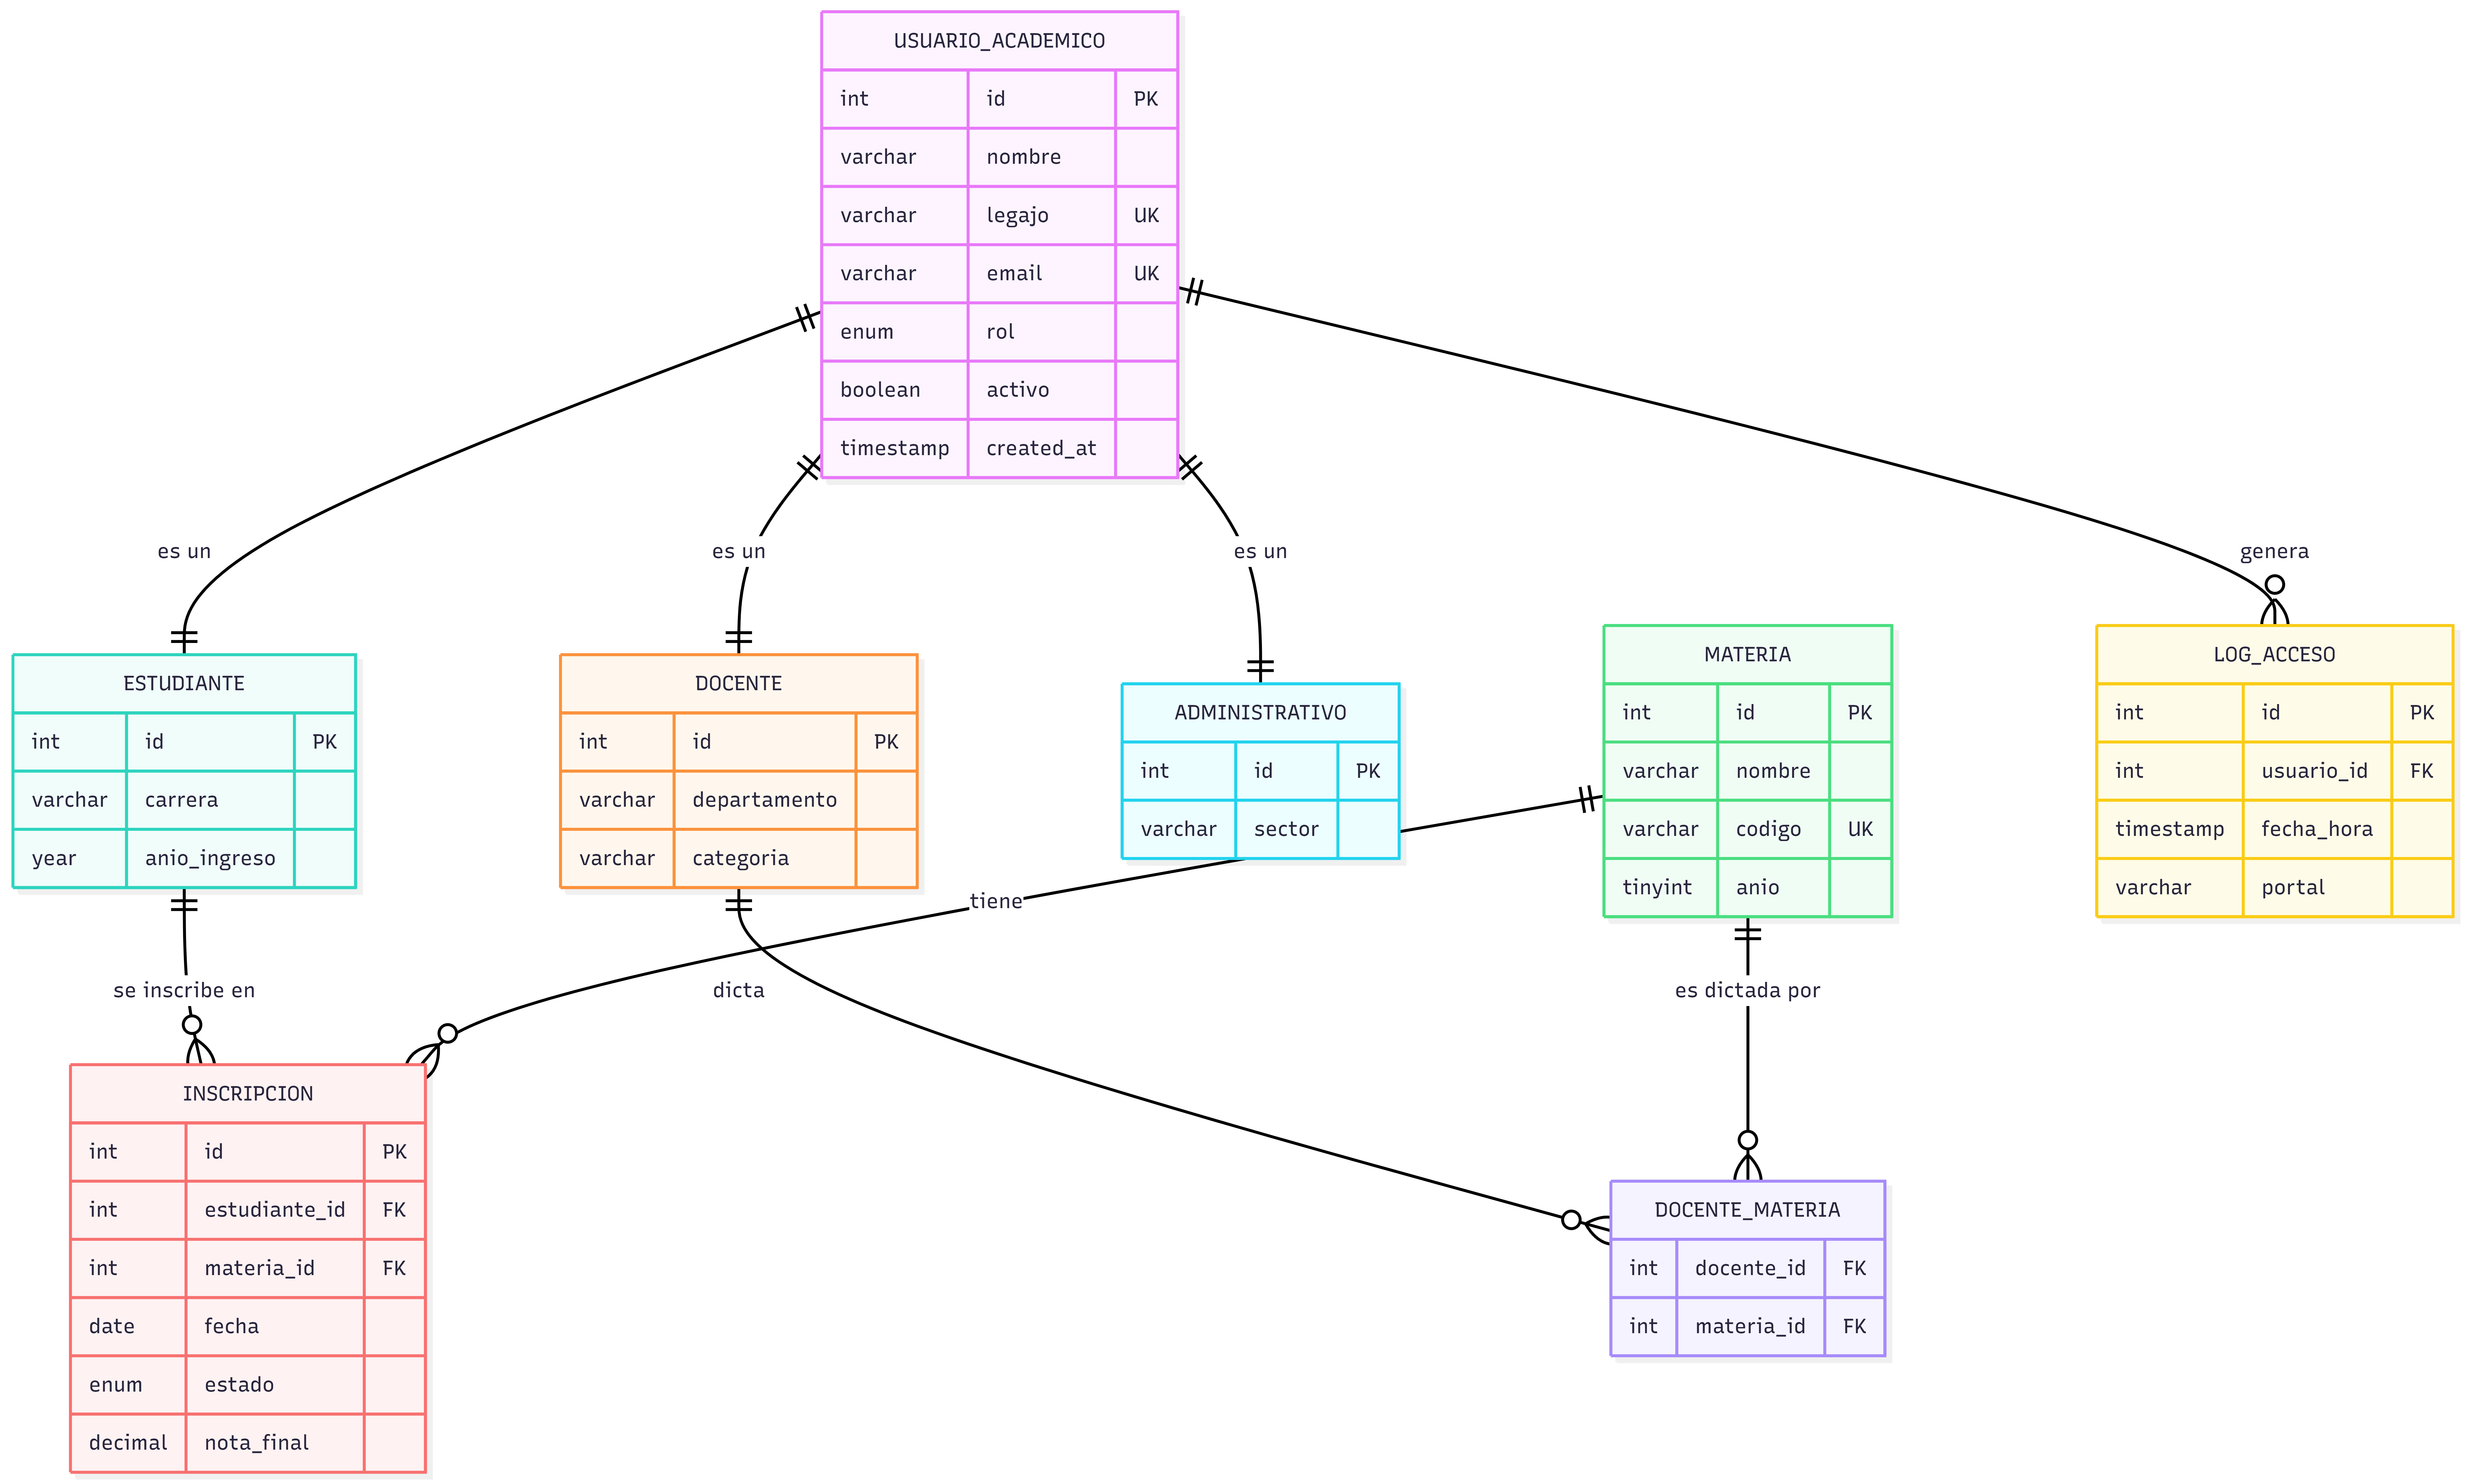
\includegraphics[width=0.92\textwidth]{../Diagrams/diagramaa.png}
    \caption{Diagrama UML de las entidades del dominio.}
    \label{fig:uml}
\end{figure}

% ======================================================================
% 6. ESTRUCTURA DEL PROYECTO
% ======================================================================
\FloatBarrier
\section{Estructura del Proyecto}

\begin{lstlisting}[language=, basicstyle=\ttfamily\footnotesize]
src/main/java/universidad/
|-- Main.java                     # Punto de entrada
|-- InputReader.java              # Lector de consola con validacion
|-- Validador.java                # Validadores estaticos reutilizables
|
|-- domain/
|   |-- UsuarioAcademico.java     # Clase base (abstracta)
|   |-- Estudiante.java           # Hereda UsuarioAcademico
|   |-- Docente.java              # Hereda UsuarioAcademico
|   |-- Administrativo.java       # Hereda UsuarioAcademico
|   |-- Materia.java              # Entidad materia
|   |-- Inscripcion.java          # Entidad inscripcion
|   |-- Nota.java                 # Value Object inmutable (0-10)
|   |-- NegocioException.java     # Excepcion de dominio
|   |-- Rol.java                  # Enum con id de DB
|   |-- CategoriaDocente.java     # Enum con id de DB
|   |-- EstadoInscripcion.java    # Enum con id de DB
|   `-- repository/
|       |-- IEstudianteRepository.java
|       |-- IDocenteRepository.java
|       |-- IAdministrativoRepository.java
|       |-- IMateriaRepository.java
|       `-- IInscripcionRepository.java
|
|-- application/
|   |-- EstudianteService.java
|   |-- DocenteService.java
|   |-- AdministrativoService.java
|   `-- InscripcionService.java
|
|-- infrastructure/
|   |-- migration/
|   |   `-- Migrator.java         # Corre SQLs en orden al iniciar
|   `-- persistence/
|       |-- ConnectionFactory.java
|       |-- EstudianteRepositoryJdbc.java
|       |-- DocenteRepositoryJdbc.java
|       |-- AdministrativoRepositoryJdbc.java
|       |-- MateriaRepositoryJdbc.java
|       `-- InscripcionRepositoryJdbc.java
|
`-- ui/menu/
    |-- MenuAlumnos.java
    |-- MenuDocentes.java
    `-- MenuAdministrativos.java

src/main/resources/db/migration/
|-- V1__schema.sql                # DDL: tablas normalizadas
`-- V2__seed.sql                  # Datos semilla

src/test/java/universidad/
`-- TestValidacionesYNota.java    # 25 tests de integracion
\end{lstlisting}

% ======================================================================
% 7. DETALLE DE IMPLEMENTACIÓN
% ======================================================================

\section{Detalle de Implementación}

\subsection{Capa de dominio: Value Object \texttt{Nota}}

\texttt{Nota} es inmutable y valida en construcción. Dos notas con el
mismo valor son iguales (por \texttt{equals} y \texttt{hashCode}), sin
necesidad de identidad.

\begin{lstlisting}[caption={Nota.java --- value object inmutable.}]
public final class Nota {

    public static final double MINIMA = 0.0;
    public static final double MAXIMA = 10.0;

    private final double valor;

    public Nota(double valor) {
        if (valor < MINIMA || valor > MAXIMA) {
            throw new IllegalArgumentException(
                "La nota debe estar entre " + MINIMA + " y " + MAXIMA + ".");
        }
        this.valor = valor;
    }

    public double getValor() { return valor; }

    @Override
    public boolean equals(Object o) {
        if (this == o) return true;
        if (!(o instanceof Nota otra)) return false;
        return Double.compare(otra.valor, valor) == 0;
    }

    @Override
    public int hashCode() { return Double.hashCode(valor); }

    @Override
    public String toString() { return String.valueOf(valor); }
}
\end{lstlisting}

\subsection{Validación por campo con \texttt{InputReader}}

Cada método de \texttt{InputReader} pide un valor y no retorna hasta que
el usuario ingresa uno válido. Esto permite corregir campos uno a uno sin
perder los ya ingresados.

\begin{lstlisting}[caption={InputReader.java --- seleccion por lista numerada.}]
public String seleccionarDeLista(String titulo, String prompt,
        List<String> valores, Function<Integer, String> resolver) {
    System.out.println(titulo);
    for (int i = 0; i < valores.size(); i++) {
        System.out.println("  " + (i + 1) + ". " + valores.get(i));
    }
    while (true) {
        System.out.print(prompt);
        String linea = scanner.nextLine().trim();
        if (linea.isEmpty()) {
            System.out.println("  Error: ingrese un numero o el valor.");
            continue;
        }
        int n;
        try { n = Integer.parseInt(linea); }
        catch (NumberFormatException e) { return linea; }
        if (n < 1 || n > valores.size()) {
            System.out.println("  Error: numero fuera de rango (1-"
                + valores.size() + ").");
            continue;
        }
        return resolver.apply(n - 1);
    }
}
\end{lstlisting}

\subsection{Persistencia con repositorios JDBC}

Cada repositorio implementa una interfaz del dominio y encapsula las
consultas SQL. Las transacciones que abarcan dos tablas (por ejemplo,
insertar en \texttt{usuario\_academico} + \texttt{estudiante}) se ejecutan
dentro de un mismo \texttt{Connection} con \texttt{commit/rollback}
manual.

\begin{lstlisting}[caption={EstudianteRepositoryJdbc --- guardar
con transaccion manual.}]
@Override
public Long guardar(UsuarioAcademico usuario, String carrera, int anio) {
    try (Connection conn = ConnectionFactory.obtener()) {
        conn.setAutoCommit(false);
        try {
            long id = insertarUsuario(conn, usuario, Rol.ESTUDIANTE);
            insertarDetalle(conn, (int) id, carrera, anio);
            conn.commit();
            return id;
        } catch (SQLException e) {
            conn.rollback();
            throw e;
        }
    } catch (SQLException e) {
        throw new NegocioException(
            "No se pudo guardar el estudiante: " + e.getMessage(), e);
    }
}
\end{lstlisting}

\subsection{Migrador de base de datos}

\texttt{Migrator} lista los archivos \texttt{.sql} ordenados por nombre y
los ejecuta secuencialmente. Funciona tanto desde el classpath de
desarrollo (\texttt{target/classes}) como desde el JAR empaquetado,
detectando el protocolo de la URL (\texttt{file:} vs \texttt{jar:}).

\subsection{Caso de uso: carga de nota}

El método \texttt{DocenteService.cargarNota} concentra las reglas de
negocio: construye un \texttt{Nota} (validación de rango), busca al
estudiante por legajo, busca la materia por código o nombre, verifica que
el alumno esté inscripto y finalmente persiste la nota.

\begin{lstlisting}[caption={DocenteService.java --- metodo cargarNota.}]
public void cargarNota(String estudianteLegajo,
        String materiaCodigoONombre, double notaValor) {
    Nota nota = new Nota(notaValor);

    var estudiante = repoEstudiantes.buscarPorLegajo(estudianteLegajo);
    if (estudiante == null) {
        throw new NegocioException(
            "El alumno con legajo '" + estudianteLegajo
            + "' no existe o no es estudiante.");
    }

    Materia materia = repoMaterias
        .buscarPorCodigoONombre(materiaCodigoONombre)
        .orElseThrow(() -> new NegocioException(
            "La materia '" + materiaCodigoONombre + "' no existe."));

    if (!repoInscripciones.existe(
            estudiante.getIdOrThrow(), materia.getId())) {
        throw new NegocioException(
            "El alumno '" + estudianteLegajo
            + "' no esta inscripto en la materia '"
            + materiaCodigoONombre + "'.");
    }

    boolean ok = repoInscripciones.actualizarNotaFinal(
        estudiante.getIdOrThrow(), materia.getId(), nota.getValor());
    if (!ok) {
        throw new NegocioException(
            "No se pudo guardar la nota. Intente nuevamente.");
    }
}
\end{lstlisting}

% ======================================================================
% 8. PATRONES DE DISEÑO APLICADOS
% ======================================================================
\section{Patrones de Diseño Aplicados}

A continuación se enumeran los patrones y principios que el proyecto aplica
de forma explícita, con una breve justificación de cada uno.

\subsection*{Arquitectura en capas (Clean Architecture)}

El proyecto separa el código en cuatro capas con dependencias
unidireccionales: la capa de dominio no importa ningún paquete de
infraestructura ni de presentación. Esto permite cambiar la base de datos o
la interfaz de usuario sin modificar las reglas de negocio.

\subsection*{SRP --- Single Responsibility Principle}

Cada clase tiene una única razón de cambio. Por ejemplo,
\texttt{DocenteService} solo contiene casos de uso relacionados con
docentes; la lógica de persistencia está en repositorios separados; la
validación de entrada está en \texttt{InputReader} y \texttt{Validador}.
Ninguna clase mezcla presentación con acceso a datos.

\subsection*{ISP --- Interface Segregation Principle}

En lugar de una interfaz genérica \texttt{IUsuarioRepository} que obligue a
todos los repositorios a implementar métodos que no necesitan, el proyecto
define cinco interfaces pequeñas y específicas:
\texttt{IEstudianteRepository}, \texttt{IDocenteRepository},
\texttt{IAdministrativoRepository}, \texttt{IMateriaRepository} e
\texttt{IInscripcionRepository}. Cada una expone solo las operaciones que
su tipo de entidad requiere.

\subsection*{DIP --- Dependency Inversion Principle}

Los servicios de aplicación (\texttt{EstudianteService},
\texttt{DocenteService}, etc.) dependen de interfaces del dominio
(\texttt{IEstudianteRepository}, \texttt{IMateriaRepository}), no de clases
concretas como \texttt{EstudianteRepositoryJdbc}. La inyección se realiza
manualmente en \texttt{Main.java}, que es el único punto que conoce las
implementaciones concretas.

\subsection*{Value Object --- \texttt{Nota}}

\texttt{Nota} es inmutable, valida su invariante en el constructor (0--10)
y su igualdad se define por valor, no por identidad. Dos instancias con el
mismo número son iguales aunque sean objetos distintos. Esto evita que una
nota inválida llegue a la base de datos y elimina la necesidad de validar
el rango en cada punto de uso.

\subsection*{Patrón de identidad nula en entidades}

Las entidades de dominio (\texttt{Estudiante}, \texttt{Docente}, etc.)
tienen un campo \texttt{Integer id} que puede ser \texttt{null} cuando el
objeto aún no fue persistido. El método \texttt{getIdOrThrow()} lanza una
excepción si se intenta usar el id antes de guardar. Esto permite
distinguir en el dominio entre ``objeto nuevo'' y ``objeto recuperado de la
base de datos'' sin contaminar las entidades con lógica de persistencia.

\subsection*{Migrador de esquema}

En lugar de depender de un ORM o de un script manual, la clase
\texttt{Migrator} recorre los archivos \texttt{.sql} del classpath en orden
alfabético y los ejecuta al iniciar la aplicación. Esto garantiza que la
base de datos siempre tenga el esquema correcto, incluso la primera vez que
se ejecuta.

\subsection*{Enum con mapeo a base de datos}

Los enums \texttt{Rol}, \texttt{CategoriaDocente} y
\texttt{EstadoInscripcion} incluyen un campo \texttt{id} que coincide con
la clave primaria de la tabla de lookup correspondiente. Los métodos
estáticos \texttt{desdeId(int)} y \texttt{desdeNombre(String)} permiten
convertir desde la base de datos al enum y viceversa, encapsulando el
mapeo en un solo lugar.

% ======================================================================
% 9. INSTRUCCIONES DE EJECUCIÓN
% ======================================================================
\section{Instrucciones de Ejecución}

\subsection{Requisitos}

\begin{itemize}
    \item \textbf{Java~17} o superior (JDK).
    \item \textbf{Maven~3.6+} (gestor de dependencias y construcción).
    \item Sistema operativo: Windows, macOS o Linux con terminal.
\end{itemize}

\subsection{Compilación}

Desde la raíz del proyecto:

\begin{lstlisting}[language=bash]
mvn clean package
\end{lstlisting}

Esto descarga la dependencia de SQLite, compila las 33 clases Java, ejecuta
los tests de integración (\emph{25 deben pasar}) y produce un JAR
auto-contenido en \texttt{target/LSP\_Universidad-1.0-SNAPSHOT.jar}.

\subsection{Ejecución}

\begin{lstlisting}[language=bash]
java -jar target/LSP_Universidad-1.0-SNAPSHOT.jar
\end{lstlisting}

La primera ejecución crea automáticamente el archivo
\texttt{resources/sistema\_universitario.db} (base SQLite) con el esquema
normalizado y los datos semilla. El menú principal aparece en la terminal.

\subsection{Ejecución de tests de integración}

\begin{lstlisting}[language=bash]
mvn dependency:build-classpath -Dmdep.outputFile=cp.txt
java -cp "target/classes:target/test-classes:$(cat cp.txt)" \
    universidad.TestValidacionesYNota
\end{lstlisting}

% ======================================================================
% 10. EVIDENCIAS DEL PROYECTO
% ======================================================================
\section{Evidencias del Proyecto}

Todo el material gráfico y audiovisual se encuentra en la carpeta
\texttt{Recursos/} dentro del directorio raíz del proyecto.

\subsection{Video de demostración de la aplicación}

Muestra el ciclo completo: inicio, migración de base de datos, alta de
alumno, inscripción a materia y carga de nota.

\begin{figure}[H]
    \centering
    \href{../Recursos/demo.mov}{\fbox{\parbox{0.5\textwidth}{\centering
        \vspace{1cm}
        {\itshape Click para abrir el video}\\[0.4em]
        {\small \texttt{Recursos/demo.mov}}
        \vspace{1cm}
    }}}
    \caption{Video demostrativo de la aplicación en ejecución.}
    \label{fig:demo}
\end{figure}

\subsection{Video de recorrido por el código y estructura}

Explica la organización en capas, los archivos principales y cómo se
conectan entre sí.

\begin{figure}[H]
    \centering
    \href{../Recursos/demo-codigo-y-estructura.mov}{\fbox{\parbox{0.5\textwidth}{\centering
        \vspace{1cm}
        {\itshape Click para abrir el video}\\[0.4em]
        {\small \texttt{Recursos/demo-codigo-y-estructura.mov}}
        \vspace{1cm}
    }}}
    \caption{Video de recorrido por el código fuente y la arquitectura.}
    \label{fig:codigo-video}
\end{figure}

\subsection{Contenido de la carpeta \texttt{Recursos/}}

La carpeta \texttt{Recursos/} contiene dos videos demostrativos (en
formato \texttt{.mov} y \texttt{.mp4}) y siete capturas de pantalla
(\texttt{.png}). Todo el material está disponible junto al código fuente
en el repositorio.

% ======================================================================
% 11. PRUEBAS Y VERIFICACIÓN
% ======================================================================
\section{Pruebas y Verificación}

\subsection{Compilación}

El proyecto compila sin errores con \texttt{mvn clean package}. El
\emph{maven-shade-plugin} produce un fat JAR con la dependencia de SQLite
embebida.

\subsection{Test de integración}

La clase \texttt{TestValidacionesYNota} ejecuta 25 casos de prueba que
cubren:

\begin{itemize}
    \item \textbf{[1] Validadores puros} (13 tests): email nulo, email sin
        arroba, email válido; campo vacío; año de ingreso fuera de rango;
        nota negativa, nota mayor a 10, nota válida.
    \item \textbf{[2] Constructores del modelo} (5 tests): nombre vacío,
        legajo vacío, email inválido, año inválido, construcción exitosa.
    \item \textbf{[3] Validaciones contra SQLite} (4 tests): legajo
        inexistente, materia inexistente, alumno no inscripto, carga
        exitosa.
    \item \textbf{[4] Persistencia real} (1 test): la nota cargada se lee
        correctamente desde otra instancia del repositorio.
    \item \textbf{[5] Listados} (2 tests): la base de datos semilla tiene
        al menos 2 estudiantes y 3 materias.
\end{itemize}

Resultado: \textbf{25/25 tests OK}.

\subsection{Smoke test manual}

Se ejecutó la aplicación con entrada simulada para verificar el flujo
completo: \texttt{1 (Alumnos) → 1 (Listar) → 0 (Volver) → 0 (Salir)}.
La aplicación listó los alumnos semilla correctamente y salió sin errores.

% ======================================================================
% 12. CONCLUSIONES
% ======================================================================
\section{Conclusiones}

El proyecto cumplió los objetivos planteados:

\begin{itemize}
    \item Se implementó un \textbf{sistema de gestión universitaria}
        en Java~17, con persistencia en SQLite, menú de consola interactivo
        y validación por campo.
    \item La \textbf{arquitectura en cuatro capas} permitió separar el
        dominio de la infraestructura y de la terminal; los servicios de
        aplicación contienen las reglas de negocio y la capa de
        infraestructura se conecta al dominio a través de interfaces.
    \item Se aplicaron los principios \textbf{SOLID}, en particular SRP,
        ISP y DIP. Las interfaces de repositorio están segregadas por tipo
        de entidad y los servicios dependen de abstracciones, no de clases
        concretas.
    \item El \textbf{esquema de base de datos} se normalizó con tablas de
        lookup, restricciones CHECK e índices sobre claves foráneas.
    \item Las listas numeradas en los menús de inscripción y carga de nota
        evitan que el usuario tenga que memorizar legajos o códigos.
\end{itemize}

% ======================================================================
% 13. TRABAJO FUTURO
% ======================================================================
\section{Trabajo Futuro}

Quedan como líneas de mejora para versiones posteriores:

\begin{itemize}
    \item \textbf{Interfaz gráfica:} reemplazar los menús de consola por
        una GUI con JavaFX o Swing, manteniendo la misma capa de dominio y
        aplicación.
    \item \textbf{Autenticación:} agregar un sistema de login con
        contraseñas hasheadas para que cada usuario acceda solo a su
        portal.
    \item \textbf{Consultas avanzadas:} historial académico del alumno
        (materias cursadas, aprobadas, promedio), reportes por docente y
        por carrera.
    \item \textbf{Cobertura de tests:} extender los tests de integración
        para cubrir los flujos de alta de docentes y administrativos, y
        agregar tests unitarios con mocks para los servicios de aplicación.
    \item \textbf{CI/CD:} configurar GitHub Actions para compilar, ejecutar
        los tests y publicar el JAR en cada push.
\end{itemize}

\end{document}
